\section{辐射度学}\label{sec:辐射度学}
 
\keyindex{辐射度学}{radiometry}{}提供了一系列描述光传播与反射的思想和数学工具。
它为贯穿本书剩余部分的渲染算法构建了推导的基础。
有趣的是,辐射度学不是用物理光学基本原理推导产生的,
而是基于穿过空间的粒子流来对光进行抽象并建立的。
因此,尽管辐射度学和\keyindex{麦克斯韦方程组}{Maxwell's equations}{}之间
已经建立了联系,为辐射度学提供了坚实的物理基础,
但像光的\keyindex{偏振}{polarization}{}
\sidenote{译者注:指横波能够朝着不同方向振荡的性质。}
那样的效应并不符合该框架。

\keyindex{辐射转移}{radiative transfer}{}是关于辐射能量转移现象的研究。
它基于辐射度量原则并在\keyindex{几何光学}{geometrical optics}{}
\sidenote{译者注:原文写作geometric optics。}层面上操作,
其中光的宏观性质足以描述光如何与比其波长大得多的物体相交。
与光的\keyindex{波动光学}{wave optics}{}模型中的现象结合并不罕见,
但这些结果需要用辐射转移的基本抽象语言来表达。
(\citet{PREISENDORFER19653}已经将辐射转移理论与
麦克斯韦描述电磁场的经典方程组联系起来。
他的框架既论证了它们的等价性又使得把一个世界观的结果应用到另一个世界观更容易了。
\citet{Fante:81}在该领域做了更多最近的工作。)

用这种方法就能描述光和与其波长大小接近的物体相交,
进而对\keyindex{色散}{dispersion}{}\sidenote{译者注:经典的棱镜色散实验。}
\begin{marginfigure}
    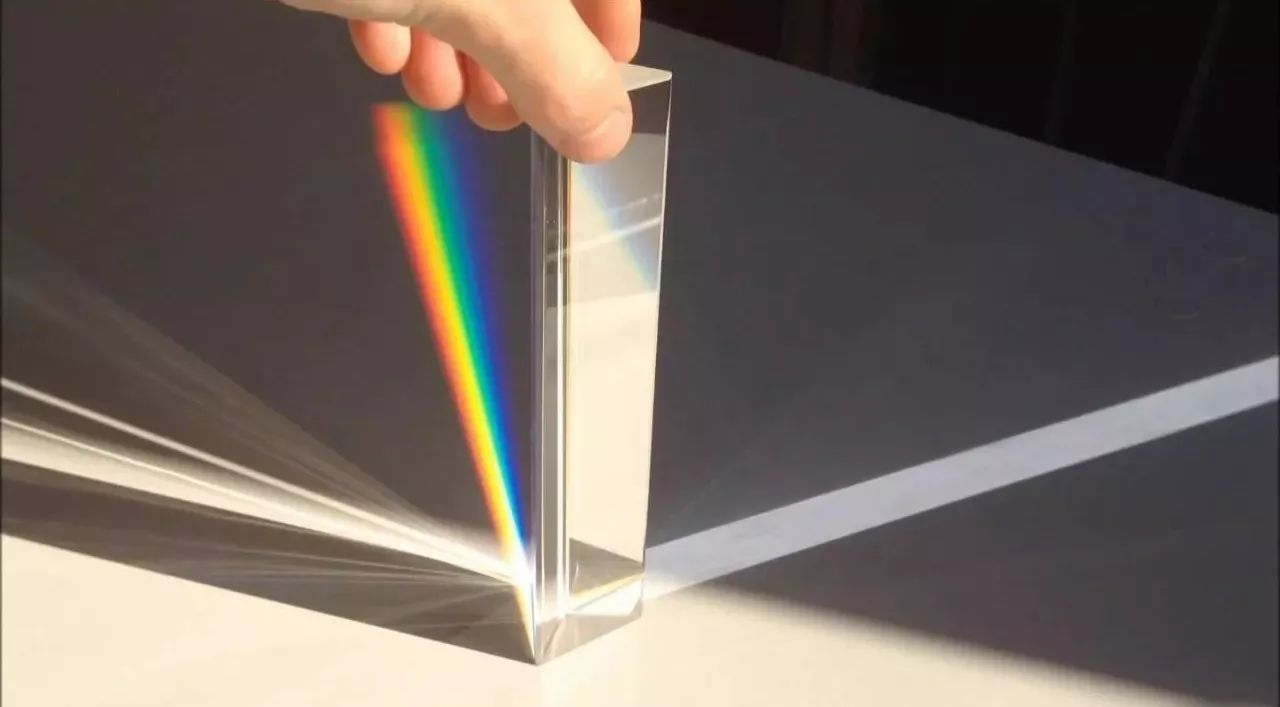
\includegraphics[width=\linewidth]{chap05/dispersion.jpg}
\end{marginfigure}
和\keyindex{干涉}{interference}{}\sidenote{译者注:经典的双缝干涉实验。}
\begin{marginfigure}
    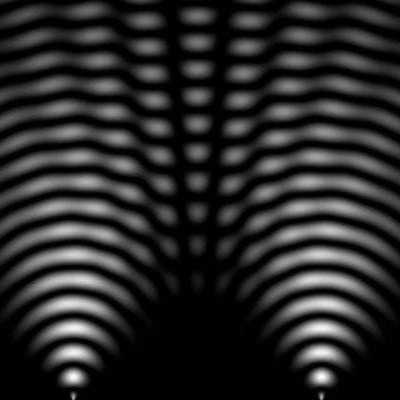
\includegraphics[width=\linewidth]{chap05/interference.jpg}
\end{marginfigure}
等效应建模。
在更精细的细节层面上,需要\keyindex{量子力学}{quantum mechanics}{}来描述光与原子的交互。
幸运的是,解决计算机图形学中的渲染问题不用直接模拟量子力学原理,
故避免了此类方法的复杂性。

在pbrt中,我们将假设几何光学是足够用来描述光与光散射的模型。
这导出了一些整个系统中隐含使用的关于光的行为的基本假设:
\begin{itemize}
    \item \keyindex{线性关系}{linearity}{}:光学系统两个输入的共同效应总是等于每个输入各自效应之和。
    \item \keyindex{能量守恒}{conservation of energy}{}\sidenote{译者注:原文写作energy conservation。}:
    当光从表面或介质散射时,触发的散射不会比它开始时产生更多的能量。
    \item {\sffamily 无偏振}:我们将忽略电磁场的偏振;
    因此,光的唯一相关属性是它关于波长(或等价地,\keyindex{频率}{frequency}{})的分布。
    \item {\sffamily 无}\keyindex{荧光}{fluorescence}{}或\keyindex{磷光}{phosphorescence}{}:
    某一波长的光的行为完全独立于其他波长或时间的光的行为。
    像偏振那样,要包含这些效应并不难,但它们为系统增加的实用价值相对较低。
    \item \keyindex{稳态}{steady state}{}:假设环境中的光达到平衡,
    所以其辐射分布不随时间变化。在现实场景中这对于光几乎是一瞬间发生的,
    所以在实践中这没什么限制。注意磷光也违反了稳态假设。
\end{itemize}

采用几何光学模型最明显的损失是很难考虑\keyindex{衍射}{diffraction}{}和干涉效应。
如\citet[p. 24]{PREISENDORFER19653}所述,这是个很难解决的问题,
例如,当存在这些效应时两区域的总通量不一定等于每个区域各自接收的功率之和。

\subsection{基本量}\label{sub:基本量}

\subsection{亮度和光度学}\label{sub:亮度和光度学}